\section{Node.js}

Node.js beroperasi sebagai lingkungan \textit{runtime} JavaScript yang bersifat asinkron dan berbasis peristiwa, yang secara khusus dirancang untuk mengembangkan aplikasi jaringan yang dapat diskalakan. Sebagai contoh, dalam skenario dasar ``\textit{Hello World}'', beberapa koneksi dapat dikelola secara bersamaan. Fungsi \textit{callback} akan dipicu untuk setiap koneksi, namun jika tidak ada tugas aktif, Node.js akan tetap dalam keadaan siaga.

\begin{figure}[htbp]
  \centering
  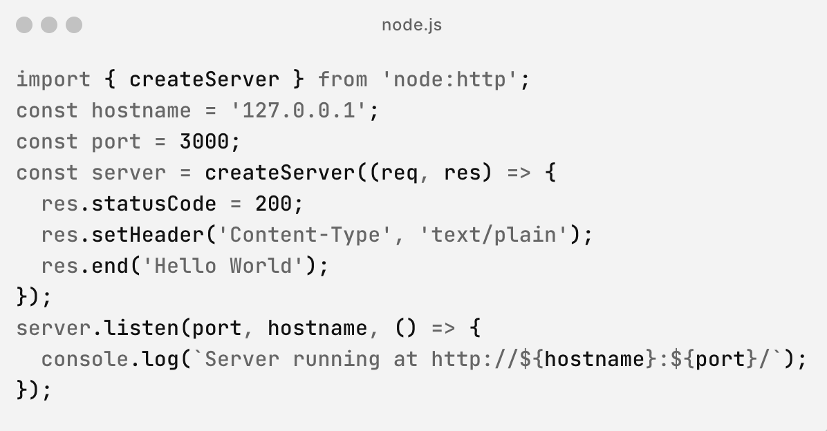
\includegraphics[width=0.85\linewidth]{images/bab-2/nodejs.png}
  \caption{Empat langkah utama untuk memproses awal dokumen untuk penggunaan LLM}\label{fig:nodejs-server}\citep{nodejs2025about}
\end{figure}

Pendekatan ini sangat berbeda dari model konkurensi tradisional yang bergantung pada \textit{thread} sistem operasi. Sistem berbasis \textit{thread} sering kali tidak efisien dan lebih sulit untuk dikelola. Node.js mengatasi masalah ini dengan menghindari penggunaan penguncian (\textit{locking}) secara keseluruhan, sehingga meminimalkan kemungkinan terjadinya kebuntuan proses. 
\singlespacing{}
Sebagian besar fungsi di Node.js tidak melakukan operasi I/O secara langsung, yang berarti prosesnya jarang mengalami pemblokiran, kecuali jika menggunakan metode sinkron dari pustaka standar Node.js. Karakteristik non-blocking ini menjadikan Node.js sangat praktis dalam pengembangan sistem yang skalabel \citep{nodejs2025about}.

\subsection{NPM}
Node Package Manager (npm) adalah utilitas penting dalam ekosistem JavaScript, yang bertindak sebagai manajer paket utama untuk lingkungan runtime Node.js. Ini menyederhanakan proses penginstalan, pengelolaan, dan pertukaran kode JavaScript, sehingga proses pengembangan menjadi lebih efisien. Repositori npm memiliki koleksi paket yang sangat banyak, berfungsi sebagai sumber daya yang berharga bagi para pengembang untuk mencari potongan kode dan pustaka yang dapat digunakan kembali. Selain itu, npm menyediakan dukungan untuk semantic versioning, sebuah sistem yang memastikan konsistensi dan kompatibilitas antara dependensi proyek. Npm meningkatkan produktivitas dan meminimalkan kemungkinan konflik atau kesalahan dalam kode dengan mengotomatiskan beberapa proses yang terkait dengan manajemen ketergantungan. Pentingnya manajemen paket ini tidak hanya untuk Node.js, karena juga digunakan dalam alur kerja pengembangan front-end, termasuk yang melibatkan kerangka kerja seperti React dan Angular \citep{nodejs2025npm}.
